\documentclass[tikz]{standalone}
\usetikzlibrary{patterns}
\usetikzlibrary{arrows}
\usetikzlibrary{decorations.shapes,decorations.markings,decorations.pathreplacing}

\tikzset{
    set arrow inside/.code={\pgfqkeys{/tikz/arrow inside}{#1}},
    set arrow inside={end/.initial=>, opt/.initial=},
    /pgf/decoration/Mark/.style={
        mark/.expanded=at position #1 with
        {
            \noexpand\arrow[\pgfkeysvalueof{/tikz/arrow inside/opt}]{\pgfkeysvalueof{/tikz/arrow inside/end}}
        }
    },
    arrow inside/.style 2 args={
        set arrow inside={#1},
        postaction={
            decorate,decoration={
                markings,Mark/.list={#2}
            }
        }
    },
}

\begin{document}
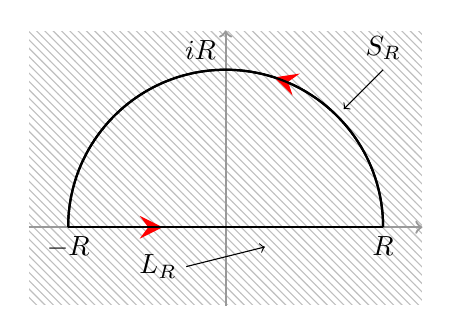
\begin{tikzpicture}
\draw[pattern=north west lines,pattern color=gray!50,draw=white] (-2.5,-1) -- (-2.5,2.5) -- (2.5,2.5) -- (2.5,-1) -- (-2.5,-1);
\draw[->,thick,color=gray!80] (-2.5,0) -- (2.5,0) ;%node[right];%{$\mathrm{Re}$};
\draw[->,thick,color=gray!80] (0,-1) -- (0,2.5) ;%node[above];%{$\mathrm{Im}$};
\draw[thick] (2,0) arc (0:180:2) [arrow inside={end=stealth,opt={red,scale=2}}{0.4}];
\draw[thick] (2,0) arc (0:180:2);
\draw[thick] (-2,0) --(2,0) [arrow inside={end=stealth,opt={red,scale=2}}{0.3}];
\draw (-2,0) node[below]{$-R$};
\draw (2,0) node[below]{$R$};
\draw[yshift=0.25cm] (0,2) node[above,left]{$iR$};
\draw[->] (-0.5,-0.5) node[left]{$L_R$} -- (0.5,-0.25);
\draw[->] (2,2) node[above]{$S_R$} -- (1.5,1.5);
\draw[thick] (-2,0) -- (2,0);
%\draw[fill=white] (0,1) circle(2pt);
%\draw (0,1) node[left]{$i$};
%\draw (0,-1) node[left]{$-i$};
%\draw[fill=white] (0,-1) circle(2pt);
\end{tikzpicture}
\end{document}